\documentclass{standalone}

\usepackage[euler-digits]{eulervm}

\usepackage{tikz}
\tikzset{every node/.style={circle,draw,minimum size=6mm,inner sep=0pt}}

\begin{document}
    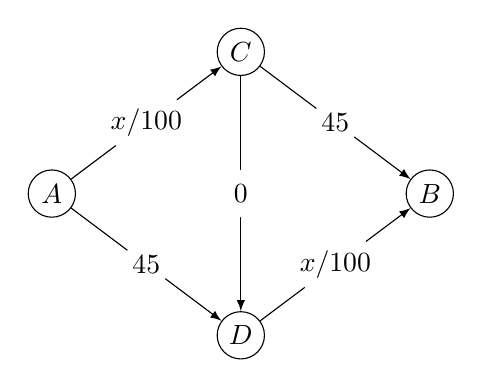
\begin{tikzpicture}[scale=1.2]
      \node (A) at (-2,0) {$A$}; 
      \node (B) at (2,0) {$B$}; 
      \node (C) at (0,1.5) {$C$}; 
      \node (D) at (0,-1.5) {$D$}; 

      \draw[->,>=latex] (A) -- node[draw=none,fill=white] {$x/100$} (C);
      \draw[->,>=latex] (D) -- node[draw=none,fill=white] {$x/100$} (B);
      \draw[->,>=latex] (A) -- node[draw=none,fill=white] {$45$} (D);
      \draw[->,>=latex] (C) -- node[draw=none,fill=white] {$45$} (B);
      \draw[->,>=latex] (C) -- node[draw=none,fill=white] {$0$} (D);
    \end{tikzpicture}
\end{document}
